\documentclass{article}

\PassOptionsToPackage{numbers,sort&compress}{natbib}
\usepackage{neurips_2026}

\usepackage[utf8]{inputenc}
\usepackage[T1]{fontenc}
\usepackage{hyperref}
\usepackage{url}
\usepackage{booktabs}
\usepackage{amsfonts}
\usepackage{amsmath}
\usepackage{amssymb}
\usepackage{microtype}
\usepackage{xcolor}
\usepackage{graphicx}
\usepackage{tikz}
\usetikzlibrary{arrows.meta,positioning,fit,backgrounds}

\hypersetup{hidelinks}

\graphicspath{{figures/}{../figures/}}

% Compact float layout. Page geometry is the unmodified NeurIPS style.
\makeatletter
\setlength{\@neuripsabovecaptionskip}{4\p@}
\makeatother
\setlength{\textfloatsep}{9pt plus 2pt minus 2pt}
\setlength{\intextsep}{8pt plus 2pt minus 2pt}
\setlength{\floatsep}{8pt plus 2pt minus 2pt}
\renewcommand{\arraystretch}{0.96}

\newcommand{\rauma}{\textsc{RauMa}}
\newcommand{\meek}{\textsc{Meek}}
\newcommand{\Dobs}{D_{\mathrm{obs}}}
\newcommand{\Dint}[1]{D^{\mathrm{int}}_{#1}}

\title{\rauma: The LLM Proposes, \meek{} Disposes for\\ Active Causal Discovery}

\author{%
  Anonymous Author(s) \\
  Affiliation \\
  Address \\
  \texttt{email} \\
}

\begin{document}

\maketitle

\begin{abstract}
Reliable scientific agents must both choose informative experiments and convert their
outcomes into valid updates of a scientific claim. End-to-end large language model (LLM)
agents entangle these roles and let unconstrained model output modify the scientific state
directly, so a final score cannot say which role failed. We separate them in active causal
discovery, where an agent spends a small intervention budget to orient an unknown causal
graph. We introduce \rauma{}, which restricts the LLM to proposing intervention targets
while a fixed mean-shift rule and \meek{} closure alone revise the graph: the model never
writes an edge. We evaluate 16 matched selector--readout configurations over 640 episodes
plus two unscaffolded baselines over 80 more, with robustness studies totalling 1{,}800
episodes. Selection is the easy half: on these small anonymized linear--Gaussian graphs
\texttt{qwen3-coder-30b} picks a target that is optimal for our structural MEC-EIG surrogate
in $93\%$ of its on-policy rounds, but a max-degree heuristic reaches $96\%$, and swapping
selectors moves directed-edge F1 by at most $0.025$. Granting an LLM terminal authority to
restate the graph from the same evidence costs $0.32$ F1. An edge-level audit localizes the
loss: both models reproduce observationally compelled arrows at the mechanical rule's own
error rate ($\approx 9\%$) while reversing $55.8\%$ and $46.5\%$ of the arrows the
experiments were run to decide, indistinguishable from coin flipping. This is not signal
detection. Auditing all 439 orientation decisions shows the two evidence classes are
perfectly separated --- true children shift by $14$--$50$ standard errors, non-children by
under $2.7$ --- and the deciding rule was stated in the readout prompt. \rauma{} reaches
$0.861$ F1 at roughly \$$0.0003$ per episode. In this benchmark, free-form belief revision
is a far larger error source than experiment selection, even when the evidence is
unambiguous.
\end{abstract}

\section{Introduction}
\label{sec:intro}

An autonomous scientific agent must close the experimental loop: identify what remains
uncertain, choose an informative experiment, and update its conclusions from the outcome.
Recent LLM systems automate increasingly large portions of that loop, but end-to-end success
conceals a distinction that matters for both science and system design. \emph{Choosing} an
experiment and \emph{interpreting} its result are different competencies with different
failure modes, and when an agent returns a wrong model a final score cannot say whether the
experiment was uninformative, the signal was missed, or valid evidence was turned into an
invalid conclusion. Adding more raw data or more tools may not resolve this if the same
generative model remains responsible for deciding what the evidence means.

\emph{Active causal discovery} is a controlled testbed for exactly that question.
Observational data identify a graph only up to its Markov equivalence class; interventions
resolve the directions observation cannot. The task exposes two modules cleanly: a
\emph{selector} chooses where to intervene under a budget, and a \emph{readout} converts the
resulting distributional changes into graph updates, so holding one fixed while varying the
other reveals which competency determines the answer. Existing active-discovery policies
choose interventions by coverage, targeted recovery, neural acquisition, Bayesian information
gain or adaptivity, and LLMs have separately served as semantic causal experts, graph-search
engines, structural priors and intervention selectors --- but both literatures report a final
graph or task score, often where variable names leak world knowledge. We anonymize the
variables to remove that shortcut and ask: \emph{where in the discovery loop is an LLM
actually useful?}

We introduce \rauma{}, a modular agent built on the principle \emph{the LLM proposes, \meek{}
disposes} (the name is not an acronym). From a partially directed graph estimated by PC it
shows the LLM a compact state --- unresolved edges, eligible targets, previous actions,
remaining budget --- and the model returns one decision: the next variable to intervene on. A
mean-shift test then orients that target's adjacent edges and \meek{} closure propagates what
acyclicity and collider constraints imply (Figure~\ref{fig:method}). The LLM never writes an
edge; every graph update is traceable to a test statistic or a graphical rule.

This allocation is a hypothesis about where LLMs help, and we test it by varying who selects
and who may state the final graph while holding environment, instances and evidence fixed. The
two axes behave very differently. Selection barely matters: the LLM usually picks a target
optimal for our information-gain surrogate, but so does a one-line max-degree rule, and the
choice moves the score by at most $0.025$ F1. The readout choice is decisive, costing $0.32$
F1, with an edge-level audit tracing the loss specifically to orientations that depend on
experimental evidence. We then close off the natural excuse for that failure: auditing every
orientation decision in the study shows true children of the intervened node shift by
$14$--$50$ standard errors and non-children by less than $2.7$, with nothing in between, and
the rule converting that gap into an arrow was stated verbatim in the readout prompt. The
models still reverse about half of these edges, and their rationales show why --- they read a
shift as evidence of a \emph{direct} edge rather than of descendance.

\rauma{} is not proposed as a stronger acquisition function. On graphs this small, exact
expected information gain runs in milliseconds and max-degree is already near-optimal, so an
LLM selector buys nothing but generality. The selector comparison is diagnostic: it
establishes that experiment selection is \emph{not} a plausible source of end-to-end failure
here, which is what makes the readout result interpretable. Our contributions, in order of
importance:
\begin{itemize}
\item \textbf{Role-factorized evaluation:} a paired factorial study --- 16 matched
selector--readout configurations over 640 episodes plus two unscaffolded baselines over 80
more --- measuring the marginal effect of \emph{choosing} and of \emph{concluding} separately
rather than reporting one end-to-end score.
\item \textbf{A localized diagnosis:} edge-level audits showing that small LLMs select
near-optimal interventions and then reverse the arrows those interventions were run to
resolve, at a chance-level rate, on statistically unambiguous evidence and under a prompt
stating the correct rule.
\item \textbf{An auditable architecture, and what it says about verifiers:} every \rauma{}
arrow is traceable to a statistic or a rule, and the same trace shows the verifier's residual
error is entirely type-I error at a conventional threshold, with the standard remedy of
abstaining under uncertainty making it worse.
\end{itemize}

\section{Method}
\label{sec:method}

\paragraph{Background.}
\label{sec:prelim}
From observational data one recovers the \emph{true DAG} $G$ only up to its Markov equivalence
class, summarized by a \emph{CPDAG} whose compelled arrows are shared by every member and whose
undirected edges remain open; orienting those edges is the agent's task. An intervention
supplies local evidence for it: under hard interventions, causal sufficiency and faithfulness,
forcing $X_a$ to an unusual value makes a distributional shift in an \emph{adjacent} $X_b$
support $a \to b$ and invariance support $b \to a$. In finite samples either decision may be
wrong, which is why we implement this below as a fixed statistical rule rather than an oracle.
\meek's rules R1--R4 then propagate what acyclicity and the absence of new colliders imply, so
one experiment can orient edges not incident to its target. We score submitted arrows with
\emph{directed-edge F1} and also report skeleton F1 (adjacencies only), compelled-edge F1 and
structural Hamming distance (SHD).

\paragraph{Problem setup and modular factorization.}
Let $G=(V,E)$ be an unknown DAG over $d$ variables from a linear--Gaussian structural causal
model (SCM)
\begin{equation}
X_i = \sum_{j \in \mathrm{Pa}_G(i)} w_{ji} X_j + \epsilon_i,
\qquad \epsilon_i \sim \mathcal{N}(0, \sigma_i^2),
\end{equation}
with independent noise and no latent confounding. A constraint-based front-end turns an
observational panel $\Dobs$ into an initial CPDAG $P_0$. At round $t$ the agent chooses a
single-node intervention $a_t$, receives a fresh panel $\Dint{t} \sim P_G(\boldsymbol{x} \mid
\mathrm{do}(X_{a_t}=v_t))$, and updates its belief graph; because the budget is small, an
uninformative choice cannot always be repaired later.

The public state is $S_t = (P_t, \boldsymbol{\mu}^{\mathrm{obs}},
\boldsymbol{s}^{\mathrm{obs}}, \mathcal{H}_t, R_t)$: per-variable observational means and
standard deviations, the history $\mathcal{H}_t$ of every experiment's target, value and
summary statistics, and the remaining budget. An episode has three replaceable components ---
a \emph{selector} $\pi$ proposing the next experiment, an online \emph{updater} $U$
maintaining the belief graph, and a terminal \emph{readout} $\rho$ producing the scored
graph:
\begin{equation}
a_t = \pi(S_t), \qquad
P_{t+1} = U\bigl(P_t, \Dobs, \Dint{t}, a_t\bigr), \qquad
\widehat{G} = \rho\bigl(P_{T+1}, P_0, \mathcal{H}_{T+1}\bigr).
\label{eq:factorization}
\end{equation}
End-to-end agents fuse all three into one conversational loop. \rauma{} is the asymmetric
composition
\begin{equation}
\rauma = \bigl(\pi_{\mathrm{LLM}},\; U_{\mathrm{MS}+\meek},\; \rho_{\mathrm{id}}\bigr),
\end{equation}
using an LLM only for $\pi$, a fixed statistical--symbolic rule for $U$, and an identity
readout $\rho_{\mathrm{id}}(P_{T+1},\cdot,\cdot)=P_{T+1}$ that submits the maintained belief
graph unchanged.

\begin{figure}[t]
\centering
\resizebox{0.93\linewidth}{!}{%
\begin{tikzpicture}[
  font=\small,
  box/.style={draw, rounded corners=2pt, align=center, inner sep=4pt, minimum height=9mm},
  llm/.style={box, fill=blue!8, draw=blue!55},
  det/.style={box, fill=black!5, draw=black!45},
  env/.style={box, fill=orange!10, draw=orange!60},
  ar/.style={-{Latex[length=2mm]}, thick, draw=black!60}
]
  \node[det] (obs) at (0,0) {$\Dobs$\\ \scriptsize observations};
  \node[det] (pc) at (2.3,0) {PC\\ \scriptsize front-end};
  \node[det] (pdag) at (4.6,0) {$P_t$\\ \scriptsize belief PDAG};
  \node[llm] (sel) at (7.5,0) {\textbf{LLM proposer}\\ \scriptsize choose target $a_t$};
  \node[env] (env) at (10.9,0) {environment\\ \scriptsize $\mathrm{do}(X_{a_t}\!=\!\bar{x}^{\mathrm{obs}}_{a_t}\!+\!3s^{\mathrm{obs}}_{a_t})$};
  \node[det] (ms) at (9.4,-2.0) {mean-shift test\\ \scriptsize $Z_{a_t\to b} > 1.96$};
  \node[det] (meek) at (5.9,-2.0) {\meek{} closure\\ \scriptsize $\mathcal{M}_{1:4}$};
  \node[det] (out) at (2.4,-2.0) {$P_{t+1}$\\ \scriptsize auditable state};

  \draw[ar] (obs) -- (pc);
  \draw[ar] (pc) -- (pdag);
  \draw[ar] (pdag) -- (sel);
  \draw[ar] (sel) -- (env);
  \draw[ar] (env) -- (ms);
  \draw[ar] (ms) -- (meek);
  \draw[ar] (meek) -- (out);
  \draw[ar] (out) -- ++(0,1.0) -| (pdag);
  \node[anchor=west, font=\scriptsize, text=blue!55] at (6.35,0.95) {one integer per round};
  \node[anchor=west, font=\scriptsize, text=black!55] at (2.9,-2.9) {graph is never written by the model};
\end{tikzpicture}}
\caption{\rauma{} separates proposal from belief revision. The LLM sees a compact structural
state and returns only an intervention target; the mean-shift test and \meek{} closure alone
determine the next graph, which \rauma{} also submits as its final output. Every arrow in
the output is traceable to a test statistic or a graphical rule.}
\label{fig:method}
\end{figure}

\paragraph{LLM experiment proposer.}
The selector receives a serialization of $S_t$: the edges of $P_t$, each node's undirected
degree, the nodes touching undecided edges, observational statistics, previous interventions
and the remaining budget. Variables are anonymized as $X_0,\dots,X_{d-1}$, and a forced tool
call returns one integer target plus a short rationale. The model is told that useful targets
touch undecided edges and that orientations may propagate, but receives neither the hidden DAG
nor a likelihood nor an enumerated class (Appendix~\ref{app:prompts} gives every prompt
verbatim). To isolate target choice from intervention magnitude, every selector uses the same
value
\begin{equation}
v_t = \bar{x}^{\mathrm{obs}}_{a_t} + 3 s^{\mathrm{obs}}_{a_t},
\end{equation}
three observational standard deviations above the mean. Selection repeats until the budget
runs out or no undirected edges remain.

\paragraph{Fixed-threshold mean-shift update.}
For each undecided neighbor $b$ of the target $a_t$, \rauma{} compares that variable's
observational and interventional means with a two-sample $z$-statistic,
\begin{equation}
Z_{a_t \to b} = \frac{\bigl|\bar{x}^{\mathrm{int}}_b - \bar{x}^{\mathrm{obs}}_b\bigr|}
{\sqrt{(s^{\mathrm{obs}}_b)^2/n_{\mathrm{obs}} + (s^{\mathrm{int}}_b)^2/n_{\mathrm{int}}}},
\qquad
o_t(a_t,b) =
\begin{cases}
a_t \to b, & Z_{a_t \to b} > 1.96,\\
b \to a_t, & \text{otherwise,}
\end{cases}
\label{eq:meanshift}
\end{equation}
over the undecided neighborhood $\mathcal{N}_u(a_t; P_t)$. Three choices matter. Restricting
the test to \emph{neighbors} preserves its local interpretation: a shift at a non-neighbor
shows only descendance, not a direct edge. Non-rejection yields the \emph{reverse}
orientation rather than an abstention, because $a_t$ and $b$ are already known to be
adjacent, so absence of a shift is itself informative. And the threshold is a fixed $1.96$
with no multiple-testing correction: the rule is a stated contract, not a calibrated
procedure. Section~\ref{sec:verifier} measures the cost of the last two choices. Writing
$\oplus$ for inserting the accepted directions and $\mathcal{M}_{1:4}$ for \meek{} closure,
\begin{equation}
P_{t+1} = \mathcal{M}_{1:4}\bigl(P_t \oplus \{o_t(a_t,b): b \in \mathcal{N}_u(a_t;P_t)\}\bigr).
\end{equation}
The rule is a finite-sample heuristic, not an oracle: pooled over all arms, $5.5\%$ of its
orientations are wrong (43 of 778, Appendix~\ref{app:ms}). Its purpose is not optimality but
a transparent evidence-to-orientation contract against which LLM interpretation can be
measured.

\paragraph{The $5\times2$ design.}
\label{sec:design}
We cross five selectors with two readouts and fix everything else. The selectors are uniform
random over open targets; maximum undirected degree; exact \emph{structural MEC-EIG}; the
\rauma{} LLM proposer; and a \emph{truth-gain reference} that greedily maximizes edges
resolved after closure under the hidden DAG. Under a uniform prior over the current class
$\mathcal{G}_t$, MEC-EIG picks the target maximizing $H(\mathcal{G}_t) - \sum_z p(z \mid a)
H(\mathcal{G}_t \mid z, a)$, where $z$ is the orientation signature of the edges touching $a$.
Every main instance has an exhaustively enumerable class (largest observed
$|\mathcal{G}_0|=28$, cap 256), so this is computed exactly --- but it remains a
\emph{structural} surrogate over graphs rather than full Bayesian design over SCM parameters,
and we keep the qualified name throughout.

The two readouts are $\rho_{\mathrm{id}}$, which submits the mechanically updated graph, and
$\rho_{\mathrm{LLM}}$, which shows an LLM the initial PC graph plus the per-experiment
sufficient statistics and takes the returned graph through a forced tool call. Critically,
the readout prompt states the intervention-to-orientation rule and the two-standard-error
convention explicitly (Appendix~\ref{app:prompts}), so we are not testing whether a model can
invent causal-discovery theory unaided. A shared sanitizer removes malformed, cyclic or
duplicated edges and logs every removal.

What makes the comparison controlled is that the online updater $U$ is the mean-shift rule in
\emph{every} grid arm, so changing the readout alters neither which experiments were run nor
what evidence reached the readout --- only which component may state the conclusion; only the
unscaffolded baseline gives the model all three roles. All grid cells share the same instances,
panels, front-end, intervention values, sample sizes, budgets and seed map. Writing $g_t(a)$
for the number of undirected edges that intervening on $a$ resolves under the hidden truth
after closure, we record \emph{selection regret} $R_{\mathrm{sel}} = \sum_t [\max_a g_t(a) -
g_t(a_t)]$ alongside directed-edge F1. Regret is computed from the hidden DAG and is never
visible to any policy but the truth-gain reference.

\section{Experimental setup}
\label{sec:setup}

\paragraph{Instances.}
The main study uses 40 paired instances, ten accepted seeds at each $(d,|E|) \in
\{(4,4),(6,6),(8,8),(10,10)\}$. Each draws a random topological order and exactly $|E|=d$
forward edges, gives every edge a coefficient of random sign and magnitude
$\mathrm{Unif}(0.5,2.0)$, and uses unit noise variance; data are not standardized. One
observational panel of $n_{\mathrm{obs}}=300$ rows is drawn per episode and reused across
rounds, while each target draws a \emph{fresh} panel of $n_{\mathrm{int}}=150$ rows under a
perfect hard intervention. The front-end is PC with Fisher-$z$ at $\alpha=0.05$; the budget is
$|I^*|+1$ for $I^*$ the minimum sufficient intervention set computed from the true DAG, giving
$2.4$ to $3.2$ interventions on average (Table~\ref{tab:ladder}).
Appendix~\ref{app:instances} gives the generator and acceptance policy in full.

Two design points invite suspicion. First, the instance filter is a \emph{non-triviality}
policy --- it rejects graphs with fewer than two undirected edges, undirected edges all
sharing one node, disconnected skeletons, near-singular covariance, or a structurally relevant
partial correlation below $0.1$ --- and never inspects the front-end's output or any policy's
score. Across the main study 122 candidates were sampled to accept 40 ($32.8\%$), and all 82
rejections came from the graph-level triviality conditions. What was tuned in advance is the
\emph{level design}: at density $|E|=d$ the PC front-end is competent but imperfect (mean
skeleton-F1 ceiling $0.938$), whereas denser graphs make PC's skeleton wrong often enough that
every arm hits the same low ceiling and the selector--readout contrast becomes unmeasurable.
Second, the true DAG lies in PC's class in only $40\%$ of instances: elsewhere the agent starts
from a CPDAG that is already partly wrong, so every arm faces an F1 ceiling below $1$. That
makes the front-end a realistic upstream component rather than an oracle, and since it applies
identically to all arms it cannot generate the contrasts we report.

\paragraph{Models and protocol.}
We evaluate two inexpensive models --- one open-weight mixture-of-experts model,
\texttt{qwen3-coder-30b-a3b-instruct}, and one proprietary compact model,
\texttt{gpt-4o-mini-2024-07-18} --- at temperature zero with forced tool calls. Every arm runs
on every instance, so all comparisons are paired; pairwise claims use two-sided Wilcoxon
signed-rank tests with win--tie--loss (W-T-L) counts, because ties are frequent and a
$p$-value alone hides them. Error bars are $95\%$ CIs, over instances for arm means and over
paired differences for contrasts. The main study is $16 \times 40 = 640$ grid episodes plus
$2 \times 40 = 80$ unscaffolded episodes; three ablations on budget, sample size and evidence
format bring the total to $1{,}800$ LLM episodes, and a model-free verifier-calibration sweep
adds no LLM cost.

\section{Results}
\label{sec:results}

\subsection{Interpretation dominates selection in the main regime}
\label{sec:main}

Table~\ref{tab:main} and Figure~\ref{fig:factorial}(a) report the arm-level results. Within
either model's five-selector comparison, arm means differ by at most $0.025$ F1, and every
mechanical arm reproduces the front-end's skeleton and compelled-edge scores exactly, because
target selection cannot alter them. Holding the selector fixed and changing only the readout
costs about $0.32$ F1 and $2.3$--$3.0$ SHD, for every selector and both models.

Because the design is factorial, each axis is best read as a marginal effect over the other.
Averaging each instance over the five selectors, the mechanical readout beats the LLM readout
by $+0.318$ for qwen3-30b ($p=7.7\times10^{-8}$, W-T-L $38$-$2$-$0$) and $+0.320$ for
gpt-4o-mini ($p=5.3\times10^{-8}$, W-T-L $39$-$1$-$0$), against a best-minus-worst selector
spread of $0.025$. In Figure~\ref{fig:factorial}(b) the readout effect ranges from $+0.279$ to
$+0.341$ across selector choices, while every selector contrast against random has an interval
containing zero; for the same LLM selector, submitting the mechanically maintained belief
graph instead of an LLM reconstruction is worth $+0.341$ (qwen) and $+0.324$ (gpt). The
unscaffolded agent, which chooses its own targets and values, keeps raw rows in context and
states its own graph, reaches $0.152$ (qwen3-30b) and $0.000$ (gpt-4o-mini); the zero is not
an infrastructure failure, as gpt-4o-mini recovers part of the skeleton but returns no
oriented edge in any of its 40 episodes. Across the 720 main episodes there were zero failed
tool calls and five schema-repair calls.

\begin{table}[t]
\caption{Main results, 40 paired instances per arm, mean $\pm$ 95\% CI. Changing the readout
(across blocks) costs roughly $0.32$ directed F1; changing the selector (within a block)
changes it by at most $0.025$. Full 18-configuration grid: Appendix~\ref{app:grid}. Token
counts are not comparable across blocks --- the unscaffolded agent receives raw rows, the
others sufficient statistics; Section~\ref{sec:robust} isolates that factor.}
\label{tab:main}
\centering
\small
\setlength{\tabcolsep}{5.0pt}
\begin{tabular}{llccccccc}
\toprule
Selector & Model & directed F1 & comp.\ F1 & skel.\ F1 & SHD & interv. & tokens & \$/ep. \\
\midrule
\multicolumn{9}{l}{\emph{mechanical readout: submit the mean-shift $+$ \meek{} belief graph}}\\
truth-gain ref. & N/A & $0.836 \pm 0.059$ & $0.925$ & $0.938$ & $1.25$ & $1.60$ & $0$ & $0$ \\
random & N/A & $0.843 \pm 0.052$ & $0.925$ & $0.938$ & $1.35$ & $1.98$ & $0$ & $0$ \\
max-degree & N/A & $0.857 \pm 0.054$ & $0.925$ & $0.938$ & $1.18$ & $1.73$ & $0$ & $0$ \\
MEC-EIG & N/A & $0.857 \pm 0.054$ & $0.925$ & $0.938$ & $1.18$ & $1.75$ & $0$ & $0$ \\
\textbf{\rauma} & qwen3-30b & $\mathbf{0.861 \pm 0.053}$ & $0.925$ & $0.938$ & $1.15$ & $1.78$ & $1{,}493$ & $0.00031$ \\
\textbf{\rauma} & gpt-4o-mini & $\mathbf{0.856 \pm 0.056}$ & $0.925$ & $0.938$ & $1.18$ & $1.83$ & $1{,}022$ & $0.00019$ \\
\midrule
\multicolumn{9}{l}{\emph{LLM readout: the model states the final graph from the same evidence}}\\
truth-gain ref. & qwen3-30b & $0.557 \pm 0.079$ & $0.914$ & $0.917$ & $3.65$ & $1.60$ & $1{,}388$ & $0.00055$ \\
truth-gain ref. & gpt-4o-mini & $0.516 \pm 0.080$ & $0.864$ & $0.830$ & $4.13$ & $1.60$ & $774$ & $0.00017$ \\
LLM & qwen3-30b & $0.520 \pm 0.088$ & $0.908$ & $0.907$ & $3.95$ & $1.78$ & $3{,}041$ & $0.00097$ \\
LLM & gpt-4o-mini & $0.533 \pm 0.088$ & $0.856$ & $0.845$ & $3.93$ & $1.83$ & $1{,}813$ & $0.00036$ \\
\midrule
\multicolumn{9}{l}{\emph{no scaffold: the model controls all three roles using raw data}}\\
LLM & qwen3-30b & $0.152 \pm 0.047$ & $0.427$ & $0.360$ & $10.48$ & $2.78$ & $52{,}033$ & $0.00749$ \\
LLM & gpt-4o-mini & $0.000 \pm 0.000$ & $0.275$ & $0.204$ & $10.50$ & $2.78$ & $35{,}404$ & $0.00365$ \\
\bottomrule
\end{tabular}
\end{table}

\begin{figure}[t]
\centering
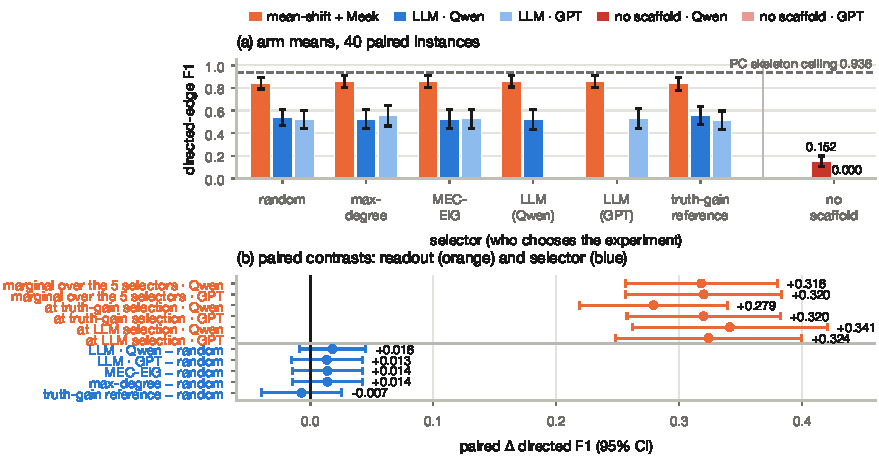
\includegraphics[width=\linewidth]{rauma_f2_factorial.pdf}
\caption{Factorial results. (a) Arm means with 95\% CIs over 40 paired instances; the dashed
line is the mean skeleton F1 attainable after the PC front-end. Two cells are absent because
each LLM selector is paired only with the readout using the same model. (b) Paired
contrasts: orange rows change only the readout, blue rows only the selector. Every blue
interval contains zero.}
\label{fig:factorial}
\end{figure}

\subsection{What the LLM readout does to individual arrows}
\label{sec:diagnosis}

An aggregate gap does not identify a mechanism, so we audit every arrow the readouts submit.
Pinning selection to the truth-gain reference makes the comparison exact: both readouts then
consume the same interventions on the same instances and see the same statistics. Each arrow
is classified as correctly oriented, reversed along a true adjacency, or spurious, then
partitioned by whether the observational CPDAG had already fixed it or the experiment was
supposed to settle it (Appendix~\ref{app:audit}).

The two readouts submit the same number of arrows for qwen3-30b (255 each), so the gap is not
abstention. The mechanical rule orients $91\%$ correctly and $8\%$ in reverse; the LLM orients
$63\%$ correctly, reverses $29\%$ and adds $7\%$ of spurious edges.
Figure~\ref{fig:readout}(b) localizes this. On arrows the front-end had already compelled, the
LLM is as reliable as the mechanical rule ($9.8\%$ versus $8.9\%$ reversed, both inherited
from PC). On arrows requiring experimental evidence, the mechanical test reverses $7.6\%$
(95\% CI $[3.7, 13.6]\%$) whereas qwen3-30b reverses $55.8\%$ ($[46.1, 65.1]\%$) and
gpt-4o-mini $46.5\%$ ($[35.7, 57.6]\%$) --- both intervals contain $50\%$, so on precisely the
edges the experiments were run to decide the models are indistinguishable from coin
flipping.

The specificity of this pattern is the point. The models do not fail at graph reasoning in
general --- they reproduce the passive-data orientations and, for qwen3-30b, the skeleton and
compelled-edge scores almost intact (Appendix~\ref{app:audit}). They fail at the one step that
converts an experiment into an arrow, and they fail there while attending to the evidence:
$80$--$100\%$ of their rationales explicitly discuss the interventions and $62$--$90\%$ mention
the observed shifts. The rationales reveal a recurring confusion between an intervention's
\emph{descendants} and its \emph{children}: ``variables whose means changed are descendants of
$X_2$; this makes $X_2$ a parent of these variables.'' That is exactly the inference the
mechanical rule is forbidden from making, because it applies the test only over the undecided
neighborhood and lets \meek{} closure handle everything further away
(Appendix~\ref{app:rationale}).

\begin{figure}[t]
\centering
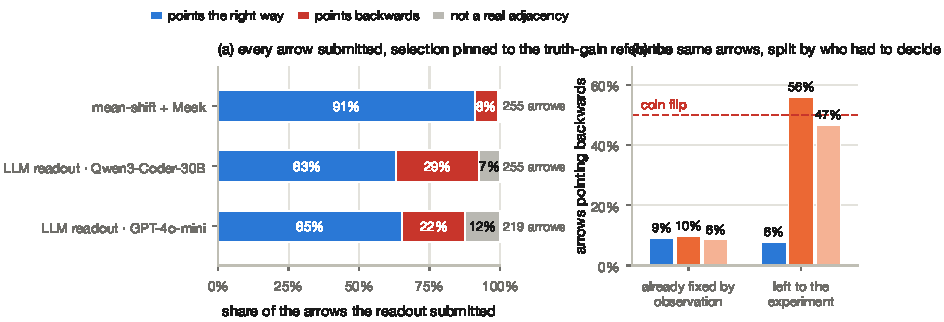
\includegraphics[width=\linewidth]{rauma_f3_readout.pdf}
\caption{Anatomy of the readout gap, with selection pinned so both readouts see identical
experiments and identical evidence. (a) Every submitted arrow is correctly oriented, reversed
along a true adjacency, or spurious. (b) The same arrows split by who had to decide the
direction. The LLM inherits the observational arrows as reliably as the mechanical rule and
orients the experiment-dependent ones at chance level.}
\label{fig:readout}
\end{figure}

\subsection{The evidence was not the hard part}
\label{sec:verifier}

A natural reading of Section~\ref{sec:diagnosis} is that interventional evidence is genuinely
noisy and small models are bad at reading it. The trace says otherwise. Replaying the
mechanical agent's decision points --- same instances, same targets, same neighborhoods,
reproducing each arm's score exactly --- and logging the $|Z|$ statistic behind all 439 of its
orientation decisions across four selectors gives Figure~\ref{fig:verifier}(a). The two classes
are perfectly separated: where the edge truly runs out of the intervened node the neighbor's
mean moves by $14.2$ to $49.9$ standard errors, and where it truly runs in, by at most $2.6$.
Nothing in the study lands in between. Two conclusions follow, in opposite directions.

\paragraph{For the LLM readout, the excuse is unavailable.} The decision is not a marginal call
between a weak effect and noise but a five-fold gap on a log scale, presented as two means and
two standard deviations, with the deciding rule and the standard-error formula written into the
readout prompt (Section~\ref{sec:design}). The models still reverse about half of these edges,
so the failure is neither signal detection nor missing domain knowledge: it is applying a
stated rule to unambiguous numbers while holding a graph in mind. That is narrower and more
actionable than ``LLMs cannot interpret experiments'', and it matches the rationales, which
misapply the rule in one direction (descendant $\Rightarrow$ child) rather than hedging about
significance.

\paragraph{For the mechanical rule, $1.96$ is the wrong number, and abstention is the wrong
fix.} The same separation shows the rule's residual error is not irreducible but entirely
type-I error at a conventional threshold: all 16 of its 439 local mistakes are non-shifts
whose noise exceeded $1.96$, and every one falls in $[1.96, 3)$. Since power against the true
alternative is effectively $1$ here, tightening the test costs no recall, and any cut in
$[2.6, 14.2]$ would be exact on this instance set: sweeping the threshold raises local
accuracy from $88.6\%$ at $z{=}1.28$ to $100\%$ at $3.29$ and directed F1 monotonically from
$0.804$ to $0.867$ (Figure~\ref{fig:verifier}(b), Appendix~\ref{app:verifier}). The standard
remedy for an imperfect verifier points the wrong way. Abstaining whenever $1.0 \leq |Z| <$
threshold makes F1 \emph{fall} from $0.848$ to $0.824$ and the error rate on the remaining
decisions \emph{rise} from $5.8\%$ to $7.7\%$, because the low-$|Z|$ band is not the
verifier's uncertain region but its most confident one --- the true $b \to a$ cases live there
and are all correct, and \meek{} closure propagates only from what is decided, so each
withheld orientation also suppresses downstream ones. Where an imperfect verifier should
abstain is a property of its error structure, not of the magnitude of its test statistic. We
nonetheless keep $1.96$ everywhere, so the readout comparison is made against a rule fixed
before the study rather than one tuned after it; \rauma{}'s reported $0.861$ understates what
its own architecture supports.

\begin{figure}[t]
\centering
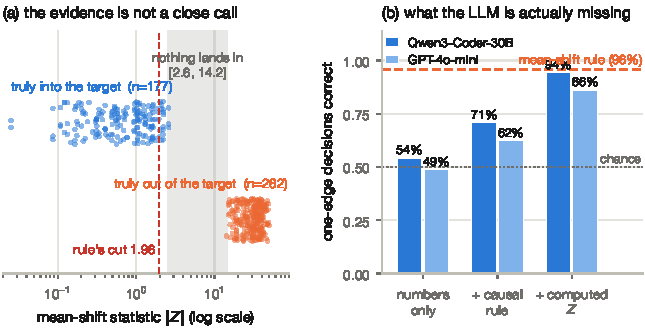
\includegraphics[width=\linewidth]{rauma_f6_verifier.pdf}
\caption{The orientation evidence is unambiguous, and the verifier's own errors are all
type-I. (a) The $|Z|$ statistic behind all 439 local orientation decisions, split by the true
direction; the classes do not overlap and nothing lands in the shaded gap. (b) Sweeping the
decision threshold: forcing an orientation improves monotonically as the test is tightened,
whereas abstaining in the low-$|Z|$ band --- which is the rule's \emph{most} reliable region
--- costs accuracy. Both panels are model-free.}
\label{fig:verifier}
\end{figure}

\subsection{The gap is not an artifact of evidence format or sample size}
\label{sec:robust}

Two explanations remain: the LLM may fail because it sees summary statistics rather than raw
data, or the rule may benefit from a sample size that flatters its $z$-test. Two ablations at
$d\in\{6,8\}$ on a fresh instance draw test both (Appendix~\ref{app:robust}). Serving the
readout raw interventional rows grows its prompt $15$--$20\times$, from $0.8$--$1.4$k to
$14$--$23$k tokens, and does not help: qwen3-30b is unmoved ($0.640 \to 0.632$), submitting the
same $6.20$ arrows per episode at the same $27.4\%$ reversal rate, while gpt-4o-mini gets
\emph{worse} ($0.603 \to 0.498$) by inventing adjacencies --- arrows per episode rise from
$5.60$ to $9.10$ and non-adjacent arrows from $9.8\%$ to $34.6\%$. Better data, by contrast,
help the rule far more than the readout: over $n_{\mathrm{obs}} \in \{60, 300, 1000\}$ the
mechanical readout moves from $0.73$ to $0.91$ F1, tracking the evidence, while the LLM readout
climbs only from $0.52$ to $0.67$, leaving a paired gap of $0.22$--$0.24$ for qwen3-30b ($p \le
6\times10^{-4}$ throughout) and $0.26$--$0.33$ for gpt-4o-mini. Seventeen times more data does
not close it, exactly as Section~\ref{sec:verifier} predicts: the quality of the statistic was
never the binding constraint.

\subsection{Selection: near-optimal choices, a small and regime-dependent payoff}
\label{sec:selection}

The other axis behaves in the opposite way: the models are good at it, and it barely matters.

\paragraph{The choices are near-optimal --- but so is a one-line heuristic.} Scoring each
round against the exact structural MEC-EIG objective, qwen3-30b picks an optimal target in
$93.0\%$ of its on-policy rounds, against $100\%$ for exact MEC-EIG by construction, $95.7\%$
for max-degree, $79.5\%$ for gpt-4o-mini and $55.7\%$ for random
(Figure~\ref{fig:selection}(a)); its selection regret is $0.225$ edges per episode versus
$1.350$ for random. Three qualifications keep the number honest: it is measured on each policy's own state
distribution, ties count as optimal, and the objective is a structural surrogate, not full
Bayesian information gain. On a stricter common-state test the LLM falls further behind
($73.7\%$ first-round agreement with MEC-EIG against $92.1\%$ for max-degree,
Appendix~\ref{app:sel}). The honest summary is that a prompted LLM is competitive with, and
slightly worse than, sorting nodes by undirected degree, while being slower and costing money.
Whether prompt-based selection stays competitive when the equivalence class is too large to
enumerate is an open question our experiments do not test.

\paragraph{The payoff is small and regime-dependent.} Figure~\ref{fig:selection}(b) shows a
nine-fold range of choice quality mapping onto a $0.025$ range of F1, because one spare
intervention usually repairs a bad choice. Removing that slack changes things: at budget
$|I^*|$ instead of $|I^*|+1$, \rauma{} exceeds random by $+0.032$ ($p=0.017$) against
$+0.018$ ($p=0.28$) in the main regime, and the gain is $+0.055$ at $n_{\mathrm{obs}}=60$
($p=0.011$) and $+0.039$ at $n_{\mathrm{obs}}=1000$ ($p=0.017$). The effect is thus small in
the main regime and larger in all three alternative regimes, largest in the data-poor one, but
not monotone in the amount of data. \rauma{} ties exact MEC-EIG in three of four regimes
($|\Delta| \leq 0.004$) and is numerically $0.028$ lower in the noisiest, which is not
significant ($p=0.11$); across twelve such comparisons the $p$-values are uncorrected and
several would not survive Bonferroni (Appendix~\ref{app:sel}).

Selection therefore contributes $0.02$--$0.08$ F1 against $0.22$--$0.32$ for interpretation:
an order of magnitude apart, with only the interpretation effect significant without degrading
the evidence. The practical consequence is a warning about evaluation --- end-to-end accuracy
is a poor diagnostic for an experiment-design policy, because a $93\%$ and a $56\%$
optimal-choice rate are nearly indistinguishable in the final score whenever the budget has
any slack.

\paragraph{Cost.} \rauma{} spends about a thousand tokens and two forced tool calls per
episode, \$$0.0003$, so restoring the scaffold is worth $+0.710$ and $+0.856$ F1 ($p<10^{-7}$)
at a thirty-fifth of the tokens (Appendix~\ref{app:cost}) --- a measure of the whole scaffold
rather than of model efficiency.

\begin{figure}[t]
\centering
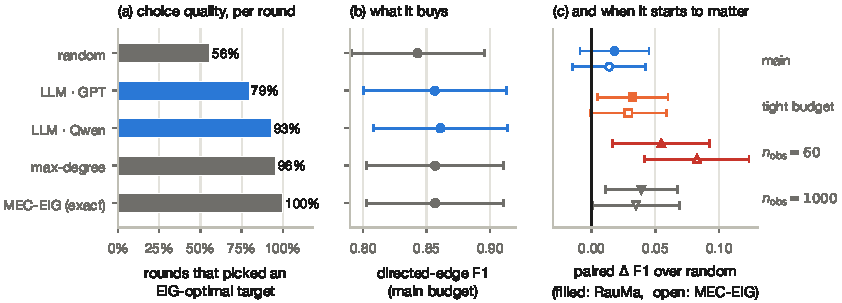
\includegraphics[width=0.8\linewidth]{rauma_f5_selection.pdf}
\caption{Choice quality and final score can be dissociated. (a) Share of rounds in which the
selector picked a target attaining the exact structural MEC-EIG optimum. (b) The resulting
directed F1, unpaired 95\% CIs, in the same order. (c) Paired gain over the random selector
in four regimes; the effect is small everywhere and separates from zero once the budget or
the data becomes scarce.}
\label{fig:selection}
\end{figure}

\section{Conclusion}
\label{sec:conclusion}

We decomposed LLM-driven active causal discovery into experiment selection and evidence
interpretation and measured both over 1{,}800 episodes. Selection is the easy half: a 30B open
model picks a target optimal for our structural MEC-EIG surrogate in $93\%$ of its rounds
without a likelihood, prior or enumerated class --- although max-degree reaches $96\%$ and the
whole axis moves the score by at most $0.025$. Interpretation is where the system breaks: on
identical evidence both models reverse roughly half of the experiment-critical arrows, and
neither raw data nor seventeen times more of it helps. The mechanism is sharper than a
capability gap, because the evidence is perfectly separable and the deciding rule was in the
prompt; the models still misapply it, in the direction their rationales describe. \rauma{}
takes the corresponding design decision --- the LLM proposes, a fixed test and \meek{} closure
dispose --- reaching $0.861$ F1 for three hundredths of a cent per episode with every arrow
traceable to a statistic or a rule.

In these small, anonymized instances the dominant measurable failure is thus not choosing what
to try but reconstructing the graph from what happened. More broadly, the boundary of model
authority mattered more than the choice between comparably small models: changing the model
moves F1 by $0.005$, whereas changing which component may state the causal conclusion moves it
by $0.32$. The same trace shows a verifier is worth auditing on its own terms --- its residual
error was a badly placed threshold, not genuine ambiguity, and the reflex of abstaining under
uncertainty made it worse.

\section*{Reproducibility statement}

All LLM results come from 1{,}800 episodes: 720 main (640 grid $+$ 80 unscaffolded), 240
tight-budget, 720 sample-size and 120 evidence-format; the verifier sweep of
Section~\ref{sec:verifier} adds eight model-free runs of 160 episodes that cost nothing to
reproduce. The release includes per-episode CSV logs, per-round step logs, per-decision orientation logs,
the full LLM call trace, a run manifest recording the seed map, and the fixed
instance-acceptance preflight. Every arm within a run shares that seed map, so all comparisons
are paired unless stated otherwise; the sample-size and evidence-format runs use a separate
instance draw and are marked unpaired where they are compared to the main study. All non-LLM
arms are deterministic --- two independent runs of 160 model-free episodes reproduced identical
scores. Both LLMs run at temperature zero with forced tool calls, and every prompt is a fixed
string reproduced in Appendix~\ref{app:prompts}. Code, logs, figure and audit scripts, the
exact command for every arm, and a script that recomputes every number in this paper are
included; the complete LLM study reruns for \$$2.39$.

\appendix

\section{Discussion}
\label{sec:discussion}

The study supports a design pattern more specific than ``use tools''. The LLM is competent at
the global, combinatorial part of the loop --- choosing an experiment from an abstract
structural description --- and unreliable at the local, rule-governed part that turns a mean
shift into an arrow. Those two facts have opposite implications for system design, and an
end-to-end score compresses them into one aggregate that supports neither. \rauma{} exploits
the asymmetry: about a thousand tokens per episode on the decision the model performs
reliably, and no model call at all for evidence interpretation. The resulting graph carries
explicit provenance, which for scientific use is not an ancillary benefit but the thing that
makes independent verification possible.

Four implications follow. First, evaluations of LLM experiment-design policies should report
choice quality against a reference objective rather than final accuracy, because
Figure~\ref{fig:selection} shows the two can be dissociated by budget slack alone. Second,
giving an agent more raw data is not a substitute for giving it a correct update rule:
Section~\ref{sec:robust} increases the readout's context by an order of magnitude with no
benefit, and Section~\ref{sec:verifier} explains why --- the statistic was never the binding
constraint. Third, the boundary of authority matters more than the choice of model within a
tier: swapping the 30B model for gpt-4o-mini changes \rauma{} by $0.005$ F1, whereas moving
the authority to state the conclusion across that boundary changes it by $0.32$. Fourth,
imperfect verifiers should be audited on their error structure rather than patched with
generic caution: here the same audit that exposed a mis-set threshold also showed that
abstaining in the low-statistic band was actively harmful, because that band was where the
verifier was right.

\section{Limitations}
\label{sec:limitations}

\textbf{Two small models.} Every claim is scoped to two inexpensive models. Frontier models
may interpret interventional evidence far better, and our results say nothing about them. The
diagnostic protocol, rather than the numerical gap, is what we expect to transfer. A useful
next step would be a single frontier readout on the same 40 logged evidence histories, which
would separate ``small models cannot do this'' from ``the authority boundary is needed
regardless of model''.

\textbf{The readout comparison still bundles two operations.} The mechanical readout decides
one edge at a time, immediately after each experiment; the LLM readout is handed the full
history at the end and must reconstruct the whole graph in one call. Our claim is therefore
about \emph{free-form terminal graph reconstruction} rather than about local evidence
interpretation in isolation. Section~\ref{sec:verifier} constrains but does not eliminate the
alternative: it shows the underlying evidence is unambiguous and the rule was supplied, so
whatever the model is failing at, it is not signal detection. A per-edge readout ablation,
which the released code supports, would close this gap directly.

\textbf{The mechanical rule is not an oracle, and the truth-gain arm is not a ceiling.} The
mean-shift rule misorients $5.5\%$ of the edges it decides, so the readout gaps are measured
against an imperfect reference and are conservative. The truth-gain arm minimizes
uninformative experiments rather than final F1, and consequently collects less evidence
($1.60$ interventions); three mechanical selectors score above it, which is why we avoid
calling it an oracle.

\textbf{The factorial surface is not additive.} The unscaffolded arm differs from \rauma{} in
several factors at once: it chooses its own intervention values, keeps raw rows in context,
and decides when to stop. The $0.32$ readout effect and the $0.71$/$0.86$ scaffold effect are
therefore not additive terms of one decomposition.

\textbf{Selection effects are small and the tests are uncorrected.} The per-regime selector
contrasts are $0.02$--$0.08$ F1 with $p$ between $0.003$ and $0.3$; across the twelve
comparisons in Table~\ref{tab:selreg} several would not survive Bonferroni. They support
``selection matters somewhat, more when evidence is scarce'', not ``selection matters a
lot''.

\textbf{The budget uses hidden information.} The budget is $|I^*|+1$, where $I^*$ is computed
from the true DAG. No policy sees $I^*$, but the benchmark still uses hidden truth to set the
resource level, which is not a deployable protocol. The tight-budget ablation
($|I^*|$) probes sensitivity to this, but a fixed budget independent of the instance would be
a cleaner design.

\textbf{The MEC-EIG reference is a structural surrogate.} It exactly optimizes the entropy of
a uniform posterior over the enumerated equivalence class, not full Bayesian experimental
design over SCM parameters, and it is tractable only because our classes are small.

\textbf{Small, sparse, synthetic, anonymized instances.} We evaluate linear--Gaussian SCMs
with $4$--$10$ nodes that are faithful by construction, have no latent confounding, and use
variable names $X_0 \dots X_{d-1}$. Largest observed equivalence class is 28 members and
typically only $2$--$5$ edges are unresolved, which is precisely why random selection is
already optimal in $56\%$ of rounds and max-degree nearly matches exact MEC-EIG. The scoped
conclusion is: \emph{in small, sparse, anonymized graphs with a competent observational
front-end and modest budget slack, selection is not the dominant bottleneck}. Anonymization
is deliberate --- it removes world-knowledge shortcuts and isolates structural reasoning ---
but it also removes the semantic prior that is arguably an LLM's main advantage in real
domains. Nonlinear mechanisms, hidden confounders, soft interventions and named variables are
untested here.

\section{Instance generation and acceptance}
\label{app:instances}

Each episode's world is built as follows, from a single seed. Sample a topological order as a
uniform permutation of $d$ nodes; enumerate the $\binom{d}{2}$ forward pairs and choose
exactly $|E|=d$ of them uniformly without replacement. Give each edge a coefficient with sign
chosen by a fair coin and magnitude $\mathrm{Unif}(0.5, 2.0)$, so $w_{ji} \in (-2,-0.5) \cup
(0.5, 2)$ --- coefficients near zero are excluded by construction, not by filtering. All
noise variances are $1.0$. Node labels are then permuted uniformly, so index order carries no
information about the topological order. Finally draw the observational panel of
$n_{\mathrm{obs}}$ rows; the panel is fixed for the whole episode and shared by every arm,
while each intervention draws a fresh panel of $n_{\mathrm{int}}$ rows under a perfect hard
intervention. Data are never standardized.

A candidate $(G, \mathrm{SCM})$ is rejected, and resampled from the same seed stream, if
(i) its CPDAG has fewer than two undirected edges, (ii) all its undirected edges share one
node, (iii) its skeleton is disconnected, (iv) its implied covariance is near singular, or
(v) any structurally relevant partial correlation has magnitude below $\epsilon = 0.1$.
Conditions (i)--(iii) exclude instances where there is nothing for an experiment to decide;
(iv)--(v) exclude near-unfaithful parameterizations. Condition (vi), that the minimum
sufficient intervention set be non-empty, is implied by (i). No condition inspects the PC
front-end, any policy's behavior, or any score.

For the main study, 122 candidates were sampled to accept 40 ($32.8\%$ acceptance), and all
82 rejections came from the graph-level triviality conditions (i)--(iii): $10/20$ at $d=4$,
$21/31$ at $d=6$, $22/32$ at $d=8$ and $29/39$ at $d=10$. No candidate was rejected by the
faithfulness margin or the intervention profile. The observational front-end is PC with a
Fisher-$z$ test at $\alpha=0.05$ as implemented in \texttt{causal-learn}; a directed part
that is not acyclic is demoted to undirected before use, which occurred in no main-study
instance. The minimum intervention set $I^*$ is the lexicographically first minimum-size set
of targets whose ideal orientation, followed by \meek{} closure, recovers the true DAG,
computed by exhaustive search over subsets. Markov equivalence classes are enumerated
exhaustively up to a cap of 256 members; the cap was never reached.

\begin{table}[h]
\caption{The instance ladder. Ten accepted seeds per level; means over instances. The
front-end is competent but imperfect, and equivalence classes are small enough for exact
MEC-EIG.}
\label{tab:ladder}
\centering
\small
\begin{tabular}{lccccccc}
\toprule
Level & $d$ & $|E|$ & $|I^*|$ & budget & PC undirected & $|\mathcal{G}_0|$ & PC skeleton-F1 ceiling \\
\midrule
0 & 4 & 4 & $1.4$ & $2.4$ & $2.6$ & $4.5$ & $0.900$ \\
1 & 6 & 6 & $1.7$ & $2.7$ & $2.6$ & $4.6$ & $0.956$ \\
2 & 8 & 8 & $1.8$ & $2.8$ & $3.3$ & $6.5$ & $0.946$ \\
3 & 10 & 10 & $2.2$ & $3.2$ & $4.6$ & $11.4$ & $0.951$ \\
\bottomrule
\end{tabular}
\end{table}

\section{Prompts}
\label{app:prompts}

Every prompt is a fixed string in the released code; only the JSON payload varies. All three
roles use forced tool calls at temperature zero, with a schema-repair retry (at most two) if
the returned arguments fail validation.

\paragraph{Selector.} System prompt:

\begin{quote}\small\ttfamily
You are the experiment-design module of a causal discovery system.\\
The world is an unknown linear-Gaussian DAG with no hidden confounders and full
observability.\\
Observational data can only identify the graph up to its Markov equivalence class: edges left
undirected in the current graph are exactly the ones observational data cannot orient.\\
An intervention do(X\_a = v) severs every incoming edge of X\_a and forces it to v. Variables
downstream of X\_a shift their mean; variables not downstream do not. Therefore intervening on
X\_a reveals the true orientation of every undirected edge incident to X\_a, and orientations
propagated from those by acyclicity and collider constraints.\\
Your job is to pick the single target that resolves the most remaining direction uncertainty.
Intervening on a variable with no incident undirected edges is a wasted experiment.\\
Call choose\_experiment exactly once.
\end{quote}

\noindent The user message is \texttt{"Session state JSON:\textbackslash n"} followed by a
compact JSON object with keys \texttt{variables}, \texttt{current\_graph}
(\texttt{directed\_edges}, \texttt{undirected\_edges}), \texttt{undirected\_degree},
\texttt{targets\_with\_open\_edges}, \texttt{observational\_stats} (\texttt{n\_rows},
\texttt{means}, \texttt{stds}), \texttt{experiments\_so\_far} (per experiment: \texttt{step},
\texttt{target}, \texttt{value}, \texttt{n\_rows}, \texttt{means}, \texttt{stds}),
\texttt{remaining\_budget} and \texttt{already\_intervened\_on}, then ``Choose the next
intervention target.'' The tool \texttt{choose\_experiment} takes an integer \texttt{target}
and a string \texttt{rationale}.

\paragraph{Readout.} System prompt:

\begin{quote}\small\ttfamily
You are the structure-inference module of a causal discovery system.\\
The world is an unknown linear-Gaussian DAG with no hidden confounders and full
observability.\\
You are given a partially oriented graph estimated from observational data, plus the results
of one or more interventions.\\
How to read an intervention do(X\_a = v): X\_a was forced to a constant, severing its incoming
edges. Compare each variable's interventional mean with its observational mean. A variable
whose mean moved is a descendant of X\_a; a variable whose mean did not move is not. For an
undirected edge \{a, b\}, a shift in X\_b under do(X\_a) means a -> b, and no shift means
b -> a.\\
Judge a shift against sampling noise: the standard error of a mean is sd / sqrt(n), so a
difference of roughly two standard errors or more is real.\\
Return a graph that is acyclic. Keep an edge undirected only if the evidence genuinely does
not orient it; leaving an edge out entirely is different from leaving it undirected.\\
Call submit\_graph exactly once.
\end{quote}

\noindent This prompt states the descendant/child distinction, the orientation rule for an
undirected edge, and a significance convention. The user message carries \texttt{variables},
\texttt{observational\_graph} (the PC CPDAG, labelled as such), \texttt{observational\_stats}
and \texttt{experiments} (the same per-experiment summaries the selector sees); in the
raw-evidence condition each experiment additionally carries its full \texttt{rows} matrix and
the observational rows are appended. The tool \texttt{submit\_graph} takes
\texttt{directed\_edges}, \texttt{undirected\_edges} and \texttt{rationale}.

\paragraph{Unscaffolded agent.} System prompt:

\begin{quote}\small\ttfamily
You are performing causal discovery over an unknown linear-Gaussian DAG with full
observability and no hidden confounders.\\
Correlation is not causation: chains and common causes create dependence between variables
that are not directly connected. Do not add an edge merely because two variables are
correlated.\\
An intervention do(X\_a = v) severs every incoming edge of X\_a and forces it to v. Variables
downstream of X\_a shift their mean; variables that are not downstream do not. Choose values
far from the observational mean so the shift is detectable.\\
Observational data alone can only identify the graph up to its Markov equivalence class, so
use your intervention budget to resolve directions.\\
The target is a directed acyclic graph. Use undirected\_edges only for genuinely unresolved
adjacencies. Take exactly one action per turn.
\end{quote}

\noindent This agent sees the raw observational rows, chooses both target and value, decides
when to stop (up to 12 turns), and submits its own graph.

\paragraph{Sanitizer.} Every LLM-produced graph passes through one shared routine before
scoring, so no arm is penalized for formatting. In order: drop entries that are not integer
pairs; drop self-loops; drop out-of-range indices; for directed edges, drop a duplicate of an
already-claimed adjacency, then drop the edge if adding it would close a cycle in what has
been accepted so far; for undirected edges, drop those overlapping an accepted directed edge
and exact duplicates. Every drop is counted and logged. Across the main study the sanitizer
removed $0.005$ cyclic and $0.31$ overlapping edges per LLM-produced graph.

\section{The full grid}
\label{app:grid}

Table~\ref{tab:grid} reports every configuration. The pattern is uniform: the six
mechanical-readout arms span $0.836$--$0.861$ directed F1 and share an identical skeleton and
compelled-edge score, while the ten LLM-readout arms span $0.516$--$0.557$ regardless of
which selector was paired with them. Two grid cells were not run because each LLM selector is
crossed only with the readout that uses the same model.

\begin{table}[h]
\caption{All 18 main-study configurations. The first 16 form the selector--readout grid; the
two unscaffolded configurations are outside the grid and reported separately. Directed F1
carries a 95\% CI over instances; the remaining columns are means.}
\label{tab:grid}
\centering
\small
\setlength{\tabcolsep}{4pt}
\begin{tabular}{llccccccc}
\toprule
Selector & Readout & directed F1 & dir.\ prec. & dir.\ rec. & comp.\ F1 & skel.\ F1 & SHD & interv. \\
\midrule
random & mech. & $0.843 \pm 0.052$ & $0.901$ & $0.798$ & $0.925$ & $0.938$ & $1.35$ & $1.98$ \\
max-degree & mech. & $0.857 \pm 0.054$ & $0.903$ & $0.820$ & $0.925$ & $0.938$ & $1.18$ & $1.73$ \\
MEC-EIG & mech. & $0.857 \pm 0.054$ & $0.903$ & $0.820$ & $0.925$ & $0.938$ & $1.18$ & $1.75$ \\
LLM (qwen) & mech. & $0.861 \pm 0.053$ & $0.907$ & $0.824$ & $0.925$ & $0.938$ & $1.15$ & $1.78$ \\
LLM (gpt) & mech. & $0.856 \pm 0.056$ & $0.902$ & $0.820$ & $0.925$ & $0.938$ & $1.18$ & $1.83$ \\
truth-gain ref. & mech. & $0.836 \pm 0.059$ & $0.878$ & $0.802$ & $0.925$ & $0.938$ & $1.25$ & $1.60$ \\
\midrule
random & LLM qwen & $0.541 \pm 0.069$ & $0.625$ & $0.504$ & $0.903$ & $0.914$ & $3.63$ & $1.98$ \\
max-degree & LLM qwen & $0.524 \pm 0.082$ & $0.629$ & $0.498$ & $0.915$ & $0.898$ & $3.85$ & $1.73$ \\
MEC-EIG & LLM qwen & $0.523 \pm 0.085$ & $0.667$ & $0.499$ & $0.915$ & $0.908$ & $4.15$ & $1.75$ \\
LLM (qwen) & LLM qwen & $0.520 \pm 0.088$ & $0.662$ & $0.482$ & $0.908$ & $0.907$ & $3.95$ & $1.78$ \\
truth-gain ref. & LLM qwen & $0.557 \pm 0.079$ & $0.641$ & $0.536$ & $0.914$ & $0.917$ & $3.65$ & $1.60$ \\
\midrule
random & LLM gpt & $0.522 \pm 0.078$ & $0.660$ & $0.462$ & $0.805$ & $0.818$ & $4.35$ & $1.98$ \\
max-degree & LLM gpt & $0.552 \pm 0.089$ & $0.640$ & $0.507$ & $0.891$ & $0.861$ & $3.63$ & $1.73$ \\
MEC-EIG & LLM gpt & $0.526 \pm 0.086$ & $0.613$ & $0.482$ & $0.885$ & $0.862$ & $4.00$ & $1.75$ \\
LLM (gpt) & LLM gpt & $0.533 \pm 0.088$ & $0.625$ & $0.485$ & $0.856$ & $0.845$ & $3.93$ & $1.83$ \\
truth-gain ref. & LLM gpt & $0.516 \pm 0.080$ & $0.628$ & $0.471$ & $0.864$ & $0.830$ & $4.13$ & $1.60$ \\
\midrule
\multicolumn{2}{l}{no scaffold (qwen)} & $0.152 \pm 0.047$ & $0.162$ & $0.144$ & $0.427$ & $0.360$ & $10.48$ & $2.78$ \\
\multicolumn{2}{l}{no scaffold (gpt)} & $0.000 \pm 0.000$ & N/A & $0.000$ & $0.275$ & $0.204$ & $10.50$ & $2.78$ \\
\bottomrule
\end{tabular}
\end{table}

Table~\ref{tab:levels} breaks the arms down by graph size and Figure~\ref{fig:scaling} plots
them. The mechanical-readout arms coincide at every $d$ and track the PC skeleton ceiling, so
\rauma{}'s residual error is dominated by the front-end and the mean-shift rule rather than
by target choice. The LLM-readout arms are $0.23$--$0.60$ lower at every graph size, with the
largest gap at $d=4$, where reversing one of four edges has the greatest proportional effect.

\begin{table}[h]
\caption{Directed F1 by level (ten paired instances each). LLM rows use qwen3-coder-30b.}
\label{tab:levels}
\centering
\small
\begin{tabular}{lcccc}
\toprule
Arm & $d=4$ & $d=6$ & $d=8$ & $d=10$ \\
\midrule
truth-gain ref., mech. & $0.700$ & $0.815$ & $0.919$ & $0.909$ \\
random, mech. & $0.757$ & $0.817$ & $0.897$ & $0.901$ \\
MEC-EIG, mech. & $0.786$ & $0.815$ & $0.907$ & $0.920$ \\
\textbf{\rauma} & $0.786$ & $0.832$ & $0.907$ & $0.920$ \\
truth-gain ref., LLM readout & $0.325$ & $0.586$ & $0.693$ & $0.623$ \\
LLM, LLM readout & $0.183$ & $0.585$ & $0.680$ & $0.631$ \\
no scaffold & $0.221$ & $0.170$ & $0.101$ & $0.113$ \\
\bottomrule
\end{tabular}
\end{table}

\begin{figure}[h]
\centering
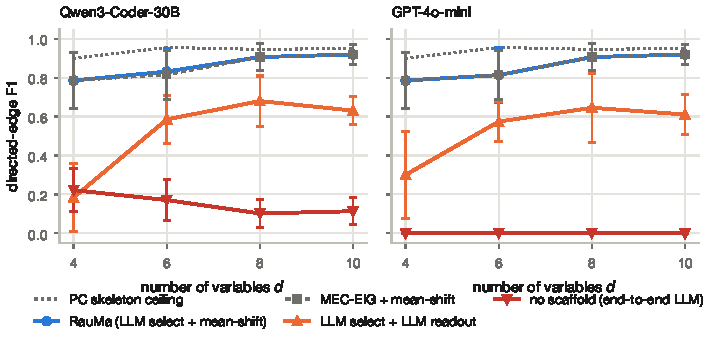
\includegraphics[width=\linewidth]{rauma_f4_scaling.pdf}
\caption{Directed F1 against the number of variables, ten paired instances per point, 95\%
CIs. The two mechanical-readout arms (blue, grey dashed) coincide at every size and stay near
the front-end ceiling; the LLM readout (orange) and the unscaffolded agent (red) are
separated from them everywhere.}
\label{fig:scaling}
\end{figure}

\section{Edge audit}
\label{app:audit}

Figure~\ref{fig:readout} is computed from the LLM call trace rather than from aggregate
metrics. For every episode we replay the deterministic components of the instance --- the
true DAG and the PC front-end, both fixed by the seed --- and extract the submitted graph
from the trace. Each submitted arrow is classified as \emph{correct} (present in the true
DAG), \emph{reversed} (its opposite is present), or \emph{spurious} (not an adjacency). It is
assigned to the \emph{observational} partition if the PC CPDAG had already oriented that
adjacency and to the \emph{experimental} partition otherwise. For the mechanical arms the
same split is recovered exactly from the episode CSV, because those arms submit no undirected
edges: directed and skeleton precision determine the three classes, and the logged number of
intervention-derived orientations determines the partition.

\begin{table}[h]
\caption{Edge audit with selection pinned to the truth-gain reference, pooled over the 40
instances. Both LLM readouts inherit the observational arrows about as reliably as the
mechanical rule and misorient about half of the experiment-dependent ones; brackets are
Clopper--Pearson 95\% intervals. All three LLM intervals contain $50\%$.}
\label{tab:audit}
\centering
\small
\setlength{\tabcolsep}{4pt}
\begin{tabular}{lcccccll}
\toprule
Readout & arrows & correct & reversed & spurious & obs.\ reversed & exp.\ reversed & 95\% CI \\
\midrule
mean-shift $+$ \meek{} & $255$ & $91.0\%$ & $8.2\%$ & $0.8\%$ & $11/124 = 8.9\%$ & $\mathbf{10/131 = 7.6\%}$ & $[3.7,\,13.6]$ \\
LLM qwen3-30b & $255$ & $63.1\%$ & $29.4\%$ & $7.5\%$ & $12/123 = 9.8\%$ & $\mathbf{63/113 = 55.8\%}$ & $[46.1,\,65.1]$ \\
LLM gpt-4o-mini & $219$ & $65.3\%$ & $22.4\%$ & $12.3\%$ & $9/106 = 8.5\%$ & $\mathbf{40/86 = 46.5\%}$ & $[35.7,\,57.6]$ \\
\bottomrule
\end{tabular}
\end{table}

Table~\ref{tab:audit_raw} repeats the audit for the evidence-format ablation. Because that
ablation runs only at $d \in \{6,8\}$, the summary rows are the corresponding main-study cells
\emph{restricted to the same two levels}, and both total arrows and arrows per episode are
reported, so the two blocks are comparable in scale. Read this way, the two models fail
differently. qwen3-30b is essentially unaffected: the same $6.20$ arrows per episode and the
same $27.4\%$ reversal rate, with a small rise in spurious edges. gpt-4o-mini becomes
\emph{denser and wronger}: $62\%$ more arrows per episode, and a third of them connecting
pairs that are not adjacent in the true graph. Neither approaches the mechanical readout. The
two runs remain separate instance draws, so this contrast is between conditions rather than
within instances.

\begin{table}[h]
\caption{Edge audit for the evidence-format ablation, selection pinned to the truth-gain
reference, $d \in \{6,8\}$, 20 instances per block. The ``summary'' rows are the main-study
cells restricted to the same two levels; the two runs are separate instance draws.}
\label{tab:audit_raw}
\centering
\small
\begin{tabular}{llccccc}
\toprule
Evidence & Model & arrows & per episode & correct & reversed & spurious \\
\midrule
summary & qwen3-30b & $124$ & $6.20$ & $69.4\%$ & $27.4\%$ & $3.2\%$ \\
raw rows & qwen3-30b & $124$ & $6.20$ & $66.9\%$ & $27.4\%$ & $5.6\%$ \\
summary & gpt-4o-mini & $112$ & $5.60$ & $70.5\%$ & $19.6\%$ & $9.8\%$ \\
raw rows & gpt-4o-mini & $182$ & $9.10$ & $41.8\%$ & $23.6\%$ & $\mathbf{34.6\%}$ \\
\bottomrule
\end{tabular}
\end{table}

Table~\ref{tab:diag} gives the same comparison in aggregate metrics. For qwen3-30b, skeleton
F1 ($0.917$ versus $0.938$) and compelled-edge F1 ($0.914$ versus $0.925$, $p=0.285$) are
largely preserved; it submits as many directed edges as the symbolic module while leaving
only $0.68$ edges undirected, so reduced directed precision is the whole story. For
gpt-4o-mini the same misorientation is compounded by edits to the front-end graph: it also
loses skeleton F1 ($-0.108$, $p=1.8\times10^{-5}$) and compelled-edge F1 ($-0.061$,
$p=0.0033$), modifying parts of the graph the evidence never touched. We therefore scope the
``preserves the CPDAG, ignores the experiments'' mechanism to qwen3-30b; for gpt-4o-mini it
comes with additional damage.

\begin{table}[h]
\caption{Readout quality with selection pinned to the truth-gain reference, so all three rows
see identical experiments and identical evidence. Figure~\ref{fig:diag} plots the same
comparison.}
\label{tab:diag}
\centering
\small
\setlength{\tabcolsep}{4.4pt}
\begin{tabular}{llcccccc}
\toprule
Readout & Model & directed F1 & dir.\ prec. & dir.\ rec. & comp.\ F1 & \#directed & \#undirected \\
\midrule
mean-shift $+$ \meek{} & N/A & $\mathbf{0.836}$ & $\mathbf{0.878}$ & $\mathbf{0.802}$ & $0.925$ & $6.38$ & $0.00$ \\
LLM & qwen3-30b & $0.557$ & $0.641$ & $0.536$ & $0.914$ & $6.38$ & $0.68$ \\
LLM & gpt-4o-mini & $0.516$ & $0.628$ & $0.471$ & $0.864$ & $5.45$ & $0.85$ \\
\bottomrule
\end{tabular}
\end{table}

\begin{figure}[h]
\centering
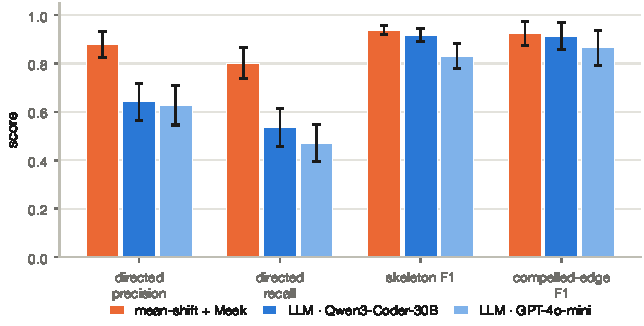
\includegraphics[width=0.9\linewidth]{rauma_a2_diagnostic.pdf}
\caption{Readout quality with selection pinned to the truth-gain reference, 95\% CIs over the
40 paired instances. The skeleton and the observationally compelled edges survive; the
orientations that require reading the interventions do not.}
\label{fig:diag}
\end{figure}

\section{Verifier calibration}
\label{app:verifier}

Section~\ref{sec:verifier} draws on two model-free measurements. The first replays the
mechanical agent on the main seed map with each of four selectors, logging every local
orientation decision together with the $|Z|$ statistic behind it. The replay reproduces the
corresponding main-study arm exactly, instance by instance, so it is a faithful substitution
point rather than a re-implementation. Pooled over the four selectors it contains 439
decisions, of which 16 are wrong ($3.6\%$). Table~\ref{tab:zbins} bins them; the emptiness
of $[3,10)$ is not a rounding artifact but the actual gap between the two evidence classes.
Those 16 local errors become 30 wrong arrows in the submitted graphs of the same four arms
($5.8\%$ of 516 orientations), because \meek{} closure faithfully propagates a wrong
premise: on average each bad local call costs about two arrows. This is why the rule's
final-graph error rate ($5.5\%$ pooled over all main arms, Appendix~\ref{app:ms}) exceeds
its decision error rate.

\begin{table}[h]
\caption{All 439 local orientation decisions of the mean-shift rule, binned by the statistic
that produced them. The rule decides $a \to b$ when $|Z| > 1.96$. Every one of its 16 errors
is a non-shift whose noise crossed the threshold, and all of them lie in $[1.96, 3)$.}
\label{tab:zbins}
\centering
\small
\begin{tabular}{lccccc}
\toprule
$|Z|$ bin & decisions & truly $a \to b$ & truly $b \to a$ & rule says $a \to b$ & errors \\
\midrule
$[0,1)$ & $103$ & $0$ & $103$ & no & $0$ \\
$[1,1.96)$ & $58$ & $0$ & $58$ & no & $0$ \\
$[1.96,3)$ & $16$ & $0$ & $16$ & yes & $\mathbf{16}$ \\
$[3,10)$ & $0$ & $0$ & $0$ & --- & $0$ \\
$\geq 10$ & $262$ & $262$ & $0$ & yes & $0$ \\
\bottomrule
\end{tabular}
\end{table}

The second measurement re-runs the four model-free selector arms with the mechanical readout
at five thresholds, and with an abstention band at three of them
(Table~\ref{tab:verifier}). Everything else is held fixed, and all runs are paired with the
main study instance by instance. Two things are worth noting. Tightening the test never costs
recall, because the number of orientations attempted is constant at 516 for every threshold
above $1.28$: with a $3$-standard-deviation intervention and coefficients bounded away from
zero, power against the true alternative is effectively $1$, so the entire operating
characteristic is driven by type-I error. And the abstention variants lose accuracy on the
decisions they still make, which is the diagnostic signature of abstaining in the wrong
region.

\begin{table}[h]
\caption{Verifier calibration sweep, four model-free selector arms $\times$ 40 instances $=$
160 episodes per row, mechanical readout, paired with the main study. ``Error rate'' is over
all orientations entering the submitted graph, including those propagated by \meek{} closure.
The abstention rows leave an edge undirected when $1.0 \leq |Z| <$ threshold.}
\label{tab:verifier}
\centering
\small
\setlength{\tabcolsep}{5pt}
\begin{tabular}{lccccc}
\toprule
Rule & directed F1 & SHD & orientations & error rate & undirected left \\
\midrule
$|Z| > 1.282$ & $0.804$ & $1.44$ & $518$ & $12.6\%$ & $0.04$ \\
$|Z| > 1.645$ & $0.837$ & $1.30$ & $516$ & $7.8\%$ & $0.05$ \\
$|Z| > 1.960$ \emph{(used throughout)} & $0.848$ & $1.24$ & $516$ & $5.8\%$ & $0.05$ \\
$|Z| > 2.576$ & $0.863$ & $1.16$ & $516$ & $3.5\%$ & $0.05$ \\
$|Z| > 3.291$ & $\mathbf{0.867}$ & $\mathbf{1.14}$ & $516$ & $\mathbf{2.7\%}$ & $0.05$ \\
\midrule
$1.645$ with abstention & $0.821$ & $1.43$ & $501$ & $9.0\%$ & $0.14$ \\
$1.960$ with abstention & $0.824$ & $1.42$ & $495$ & $7.7\%$ & $0.18$ \\
$2.576$ with abstention & $0.831$ & $1.37$ & $493$ & $5.7\%$ & $0.19$ \\
\bottomrule
\end{tabular}
\end{table}

We keep $1.96$ in every reported result. The threshold was fixed before the study, and
re-tuning the reference after seeing that it beats the LLM readout would weaken exactly the
comparison the paper is about. The honest statement is that the reference \rauma{} is
measured against is conservative by roughly $0.02$ F1.

\section{Robustness ablations}
\label{app:robust}

All three ablations reuse the study's machinery unchanged and differ from the main run in one
setting each. The tight-budget run shares the main seed map, so it pairs with the main study
instance by instance; the sample-size and evidence-format runs share a different seed map with
each other, so they pair among themselves but not with the main study. Contrasts crossing that
boundary are marked unpaired and use Mann--Whitney tests. The runner now accepts
\texttt{-\/-seed-map-from}, so future ablations can borrow the main seed map directly and stay
paired.

\paragraph{Tight budget.}
Cutting the budget from $|I^*|+1$ to $|I^*|$ removes the extra experiment that compensates for
a suboptimal target; budget slack plays no part in instance acceptance, so the graphs are
identical to the main run. Arm means fall to random $0.809$, LLM (gpt) $0.831$, truth-gain
$0.833$, max-degree $0.837$, MEC-EIG $0.838$ and LLM (qwen) $0.841$. Every arm loses accuracy
but random loses most, which is direct evidence that the small selector differences of the
main study come partly from budget slack rather than from equivalent selection quality.

\paragraph{Sample size.}
Table~\ref{tab:nsweep} sweeps $(n_{\mathrm{obs}}, n_{\mathrm{int}})$ over $(60,40)$,
$(300,150)$ and $(1000,500)$ at $d \in \{6,8\}$. The mechanical readout tracks the quality of
the evidence; the LLM readout improves far more slowly, leaving a gap that varies by at most
$0.02$ for qwen3-30b across a $17\times$ range.

\begin{table}[h]
\caption{Sample-size sweep, $d \in \{6,8\}$, 20 instances per cell, marginal over the five
selectors. The $n=60$ and $n=1000$ rows are paired with each other; the $n=300$ row is the
main study restricted to the same two levels and is a separate instance draw. $\Delta$ is the
paired mechanical-minus-LLM difference within each run.}
\label{tab:nsweep}
\centering
\small
\setlength{\tabcolsep}{4.7pt}
\begin{tabular}{lccccc}
\toprule
$n_{\mathrm{obs}}/n_{\mathrm{int}}$ & PC skel.\ F1 & mean-shift error & mech.\ readout & LLM readout (qwen) & $\Delta$ ($p$) \\
\midrule
$60/40$ & $0.831$ & $9.5\%$ & $0.732$ & $0.516$ & $+0.216$ ($6.0{\times}10^{-4}$) \\
$300/150$ & $0.951$ & $7.7\%$ & $0.863$ & $0.628$ & $+0.235$ ($1.3{\times}10^{-4}$) \\
$1000/500$ & $0.981$ & $5.5\%$ & $0.908$ & $0.673$ & $+0.235$ ($2.1{\times}10^{-4}$) \\
\bottomrule
\end{tabular}
\end{table}

Table~\ref{tab:nsweep_arms} gives all 18 configurations of both sample-size runs. The ordering
is consistent with the main study at both ends of the sweep, and the LLM-readout arms of both
models move together. The unscaffolded agent gives the most direct evidence that data volume
is not the binding constraint: at $n_{\mathrm{obs}}=1000$ it consumes $105$k tokens per
episode for gpt-4o-mini and $153$k for qwen3-30b, roughly three times its $n=60$ context, yet
its score does not improve --- gpt-4o-mini stays at $0.000$ and qwen3-30b moves from $0.203$
to $0.152$.

\begin{table}[h]
\caption{Directed F1 for all 18 configurations of the two sample-size runs, $d \in \{6,8\}$,
20 paired instances each. LLM-readout arms are labelled by the readout model.}
\label{tab:nsweep_arms}
\centering
\small
\begin{tabular}{lcc@{\hskip 16pt}lcc}
\toprule
Arm & $n{=}60$ & $n{=}1000$ & Arm & $n{=}60$ & $n{=}1000$ \\
\midrule
random, mech. & $0.679$ & $0.879$ & random, LLM qwen & $0.501$ & $0.633$ \\
max-degree, mech. & $0.761$ & $0.919$ & max-degree, LLM qwen & $0.517$ & $0.668$ \\
MEC-EIG, mech. & $0.761$ & $0.914$ & MEC-EIG, LLM qwen & $0.541$ & $0.677$ \\
\rauma{} (qwen) & $0.733$ & $0.918$ & LLM (qwen), LLM qwen & $0.507$ & $0.704$ \\
\rauma{} (gpt) & $0.749$ & $0.917$ & truth-gain ref., LLM qwen & $0.514$ & $0.682$ \\
truth-gain ref., mech. & $0.727$ & $0.912$ & random, LLM gpt & $0.425$ & $0.595$ \\
no scaffold (qwen) & $0.203$ & $0.152$ & max-degree, LLM gpt & $0.396$ & $0.624$ \\
no scaffold (gpt) & $0.000$ & $0.000$ & MEC-EIG, LLM gpt & $0.384$ & $0.627$ \\
 & & & LLM (gpt), LLM gpt & $0.415$ & $0.643$ \\
 & & & truth-gain ref., LLM gpt & $0.417$ & $0.644$ \\
\bottomrule
\end{tabular}
\end{table}

\begin{figure}[h]
\centering
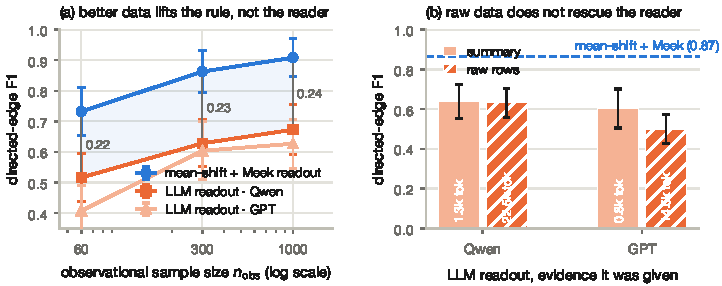
\includegraphics[width=0.8\linewidth]{rauma_f4_robust.pdf}
\caption{The readout gap survives both alternative explanations. (a) Directed F1 as the
observational panel grows, marginal over the five selectors, $d \in \{6,8\}$; annotations are
paired mechanical-minus-LLM differences for qwen3. (b) The LLM readout given sufficient
statistics versus raw interventional rows, with prompt sizes; the dashed line is the
mechanical readout on the same ladder levels.}
\label{fig:robust}
\end{figure}

\paragraph{Evidence format.}
Table~\ref{tab:raw} replaces the per-experiment sufficient statistics in the readout prompt
with the raw interventional rows. qwen3-30b is unchanged; gpt-4o-mini loses about $0.11$ F1,
and Table~\ref{tab:audit_raw} attributes that loss to invented adjacencies rather than to
misread shifts.

\begin{table}[h]
\caption{Sufficient statistics versus raw interventional rows for the LLM readout, $d \in
\{6,8\}$, 20 instances per cell. Summary columns are the main study restricted to the same two
levels; the two runs are separate instance draws, so the contrast is unpaired
(Mann--Whitney). The mechanical readout on the corresponding main instances scores $0.864$.}
\label{tab:raw}
\centering
\small
\begin{tabular}{llcccc}
\toprule
Selector & Model & summary F1 (tokens) & raw F1 (tokens) & $\Delta$ & $p$ \\
\midrule
truth-gain ref. & qwen3-30b & $0.640$ ($1.3$k) & $0.632$ ($22.5$k) & $-0.008$ & $0.97$ \\
MEC-EIG & qwen3-30b & $0.643$ ($1.4$k) & $0.632$ ($22.9$k) & $-0.011$ & $0.82$ \\
LLM & qwen3-30b & $0.633$ ($2.9$k) & $0.635$ ($23.6$k) & $+0.003$ & $0.91$ \\
truth-gain ref. & gpt-4o-mini & $0.603$ ($0.8$k) & $0.498$ ($14.5$k) & $-0.105$ & $0.05$ \\
MEC-EIG & gpt-4o-mini & $0.592$ ($0.8$k) & $0.474$ ($15.4$k) & $-0.118$ & $0.05$ \\
LLM & gpt-4o-mini & $0.610$ ($1.8$k) & $0.507$ ($16.5$k) & $-0.103$ & $0.13$ \\
\bottomrule
\end{tabular}
\end{table}

\section{Selection quality}
\label{app:sel}

Table~\ref{tab:sel} gives the per-episode selection diagnostics behind
Figure~\ref{fig:selection}(a), and Table~\ref{tab:selreg} the paired contrasts behind panel
(c). Regret, quality and MEC-EIG regret are computed by the benchmark from the hidden DAG and
are invisible to every policy except the truth-gain reference.

\begin{table}[h]
\caption{Selection quality with the readout held mechanical, main study. ``MEC-EIG-optimal
rounds'' is the share of rounds in which the chosen target attained the maximum of the exact
structural MEC-EIG objective, measured on each policy's own state distribution; ties count as
optimal. A 30B open model is close to exact MEC-EIG and far from random --- and slightly
behind max-degree --- yet the final F1 barely moves.}
\label{tab:sel}
\centering
\small
\begin{tabular}{llccccc}
\toprule
Selector & Model & directed F1 & regret & EIG regret (nats) & EIG-optimal rounds & interv. \\
\midrule
random & N/A & $0.843$ & $1.350$ & $0.401$ & $55.7\%$ & $1.98$ \\
LLM & gpt-4o-mini & $0.856$ & $0.450$ & $0.128$ & $79.5\%$ & $1.83$ \\
LLM & qwen3-30b & $\mathbf{0.861}$ & $0.225$ & $0.028$ & $93.0\%$ & $1.78$ \\
MEC-EIG & N/A & $0.857$ & $0.175$ & $0.000$ & $100\%$ & $1.75$ \\
max-degree & N/A & $0.857$ & $0.150$ & $0.007$ & $\mathbf{95.7\%}$ & $1.73$ \\
truth-gain ref. & N/A & $0.836$ & $0.000$ & $0.139$ & $79.7\%$ & $1.60$ \\
\bottomrule
\end{tabular}
\end{table}

\begin{table}[h]
\caption{Paired contrasts on the selector axis in four evidence regimes, readout held
mechanical. Effects are small everywhere; they grow and become significant once the budget or
the sample size is cut, but not monotonically in the amount of data. $p$-values are
uncorrected.}
\label{tab:selreg}
\centering
\small
\begin{tabular}{lcccc}
\toprule
Comparison & main & tight budget & $n_{\mathrm{obs}}{=}60$ & $n_{\mathrm{obs}}{=}1000$ \\
\midrule
\rauma{} (qwen) $-$ random & $+0.018$ ($0.28$) & $+0.032$ ($0.017$) & $+0.055$ ($0.011$) & $+0.039$ ($0.017$) \\
MEC-EIG $-$ random & $+0.014$ ($0.53$) & $+0.029$ ($0.061$) & $+0.083$ ($0.003$) & $+0.035$ ($0.065$) \\
max-degree $-$ random & $+0.014$ ($0.53$) & $+0.028$ ($0.10$) & $+0.083$ ($0.003$) & $+0.040$ ($0.017$) \\
\rauma{} (qwen) $-$ MEC-EIG & $+0.004$ ($0.32$) & $+0.003$ ($0.50$) & $-0.028$ ($0.11$) & $+0.004$ ($0.47$) \\
\bottomrule
\end{tabular}
\end{table}

Table~\ref{tab:roundreg} repeats the per-round measurement in the other three regimes. It is
the most stable quantity in the study: qwen3-30b stays between $89\%$ and $94\%$ optimal,
max-degree between $94\%$ and $97\%$, and random varies between $35\%$ and $56\%$ depending on
how many targets are open. The final-score contrasts of Table~\ref{tab:selreg} move by a
factor of three across the same four regimes while these rates barely move, which is the
cleanest statement of the dissociation: choice quality and downstream score are measuring
different things.

\begin{table}[h]
\caption{Share of rounds in which the selector picked a target attaining the exact structural
MEC-EIG optimum, in all four regimes (round counts in brackets). Ties count as optimal, so
MEC-EIG is $100\%$ by construction, and each row is measured on its own policy's states.}
\label{tab:roundreg}
\centering
\small
\begin{tabular}{lcccc}
\toprule
Selector & main & tight budget & $n_{\mathrm{obs}}{=}60$ & $n_{\mathrm{obs}}{=}1000$ \\
\midrule
random & $55.7\%$ (79) & $52.3\%$ (65) & $35.1\%$ (37) & $37.5\%$ (40) \\
LLM gpt-4o-mini & $79.5\%$ (73) & $76.9\%$ (65) & $87.5\%$ (32) & $91.7\%$ (36) \\
LLM qwen3-30b & $93.0\%$ (71) & $93.8\%$ (64) & $90.3\%$ (31) & $89.2\%$ (37) \\
max-degree & $\mathbf{95.7\%}$ (69) & $\mathbf{95.3\%}$ (64) & $\mathbf{96.9\%}$ (32) & $\mathbf{94.4\%}$ (36) \\
MEC-EIG & $100\%$ (70) & $100\%$ (64) & $100\%$ (33) & $100\%$ (36) \\
\bottomrule
\end{tabular}
\end{table}

A stricter check compares the targets chosen in the first round, when every selector observes
an identical state. Among the 38 main instances with at least one undecided edge, the LLM
proposer picks the same variable as exact MEC-EIG in $28$ cases ($73.7\%$) for qwen3-30b and
$26$ ($68.4\%$) for gpt-4o-mini, against $35$ ($92.1\%$) for max-degree and $9$ ($23.7\%$) for
random. Exact agreement is lower than optimality because the objective often has ties broken
differently by the two rules; the truth-gain reference, which optimizes a different objective
altogether, also agrees only $68.4\%$ of the time. On this common-state comparison the LLM is
clearly behind max-degree, which is the honest way to read the $93\%$ headline.

\section{Cost accounting}
\label{app:cost}

Table~\ref{tab:cost} gives the per-episode budget of every LLM configuration and
Figure~\ref{fig:cost} plots accuracy against context size.

\begin{table}[h]
\caption{Cost per episode. \rauma{} reaches about $0.86$ directed F1 on roughly one thousand
tokens and two forced tool calls, whereas end-to-end prompting uses about thirty-five thousand
tokens for near-zero F1. Prices are OpenRouter list prices at the time of the run, frozen in
the released manifest.}
\label{tab:cost}
\centering
\small
\begin{tabular}{llccccc}
\toprule
Arm & Model & prompt tok. & completion tok. & LLM calls & \$/episode & directed F1 \\
\midrule
\textbf{\rauma} & gpt-4o-mini & $944$ & $78$ & $1.83$ & $0.00019$ & $0.856$ \\
\textbf{\rauma} & qwen3-30b & $1{,}395$ & $98$ & $1.78$ & $0.00031$ & $\mathbf{0.861}$ \\
LLM sel.\ $+$ LLM readout & gpt-4o-mini & $1{,}618$ & $195$ & $2.83$ & $0.00036$ & $0.533$ \\
LLM sel.\ $+$ LLM readout & qwen3-30b & $2{,}497$ & $543$ & $2.83$ & $0.00097$ & $0.520$ \\
no scaffold & gpt-4o-mini & $35{,}163$ & $241$ & $3.78$ & $0.00365$ & $0.000$ \\
no scaffold & qwen3-30b & $51{,}556$ & $477$ & $3.78$ & $0.00749$ & $0.152$ \\
\bottomrule
\end{tabular}
\end{table}

Reliability was not a confound: across all 720 main episodes there were zero failed tool calls
and five schema-repair calls, and the sanitizer dropped $0.005$ cyclic and $0.31$ overlapping
edges per LLM-produced graph. The main study cost \$$0.64$ and $4.15$M tokens; all $1{,}800$
LLM episodes together cost \$$2.39$ and $12.7$M tokens. The verifier sweep of
Appendix~\ref{app:verifier} is model-free and free.

\begin{figure}[h]
\centering
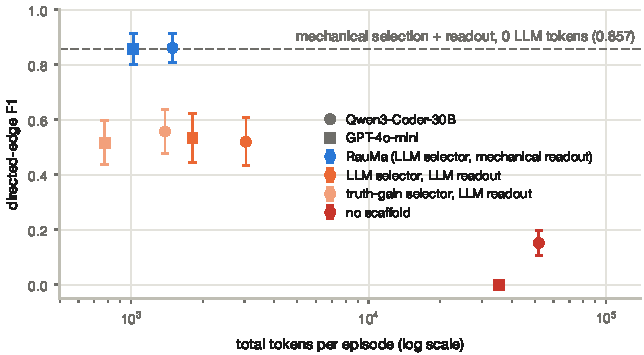
\includegraphics[width=0.86\linewidth]{rauma_a1_cost.pdf}
\caption{Token use against directed-edge accuracy, logarithmic $x$-axis, 95\% CIs over
instances. More raw data in context does not move the agents toward the mechanical reference.
The two least expensive LLM configurations perform best, matching the accuracy of the
zero-token mechanical baseline.}
\label{fig:cost}
\end{figure}

\section{Mean-shift orientation errors}
\label{app:ms}

Pooled over all main-study arms the mean-shift rule produced 778 orientations of which 43 were
wrong ($5.5\%$): $6.4\%$ at $d=4$, $10.9\%$ at $d=6$, $5.1\%$ at $d=8$ and $2.2\%$ at $d=10$
(Figure~\ref{fig:ms}). The rate is not monotone in graph size. Appendix~\ref{app:verifier}
identifies the source: in the four arms whose decisions we replayed, every underlying local
error is a type-I error in the narrow band $[1.96, 3)$, so the rate reflects how many null decisions a level happens to require and how
much closure amplifies each mistake, not a growing difficulty in reading the evidence. This is
the dominant residual error of \rauma{}, and the sweep shows most of it is removable by moving
the threshold.

\begin{figure}[h]
\centering
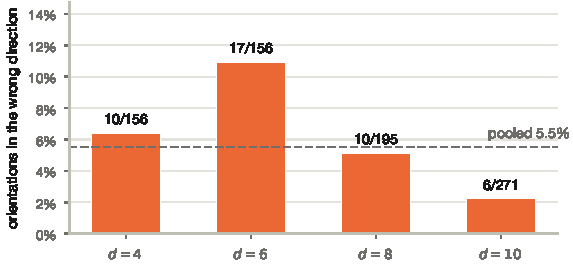
\includegraphics[width=0.68\linewidth]{rauma_a3_meanshift.pdf}
\caption{Fraction of incorrect mean-shift orientations by graph size, with counts above each
bar.}
\label{fig:ms}
\end{figure}

\section{Readout rationales}
\label{app:rationale}

Every LLM readout call is logged with the rationale returned alongside the graph. Across the
400 readout episodes of the main study (405 calls including five schema repairs), $80\%$
(qwen3-30b) and $100\%$ (gpt-4o-mini) explicitly discuss the interventions and $62\%$ /
$90\%$ mention the observed mean shifts. The failure of Section~\ref{sec:diagnosis} is
therefore not explained by simple omission of the interventions from the generated
rationales. The recurring error is a confusion between the descendants of an intervention and
its children. Two verbatim examples, lightly truncated:

\begin{quote}\small
``The intervention on $X_2$ affects the means of $X_0$, $X_1$, $X_3$, $X_4$, $X_5$, $X_6$ and
$X_7$. Variables whose means changed are descendants of $X_2$. \emph{This makes $X_2$ a
parent of these variables.}'' \hfill (qwen3-coder-30b, $d=8$)
\end{quote}

\begin{quote}\small
``The directed edges are based on the observed shifts in means after interventions. $X_0$
influences all other variables, and the relationships are consistent with the observed
data.'' \hfill (gpt-4o-mini, $d=10$)
\end{quote}

\begin{table}[h]
\caption{Content of the readout rationales over the 405 readout calls in the main study. The
models mention the evidence but often convert it into an incorrect graphical claim.}
\label{tab:rationale}
\centering
\small
\begin{tabular}{lcccc}
\toprule
Model & calls & mentions the interventions & mentions the observed shifts & mean length \\
\midrule
qwen3-coder-30b & $205$ & $80\%$ & $62\%$ & $782$ chars \\
gpt-4o-mini & $200$ & $100\%$ & $90\%$ & $313$ chars \\
\bottomrule
\end{tabular}
\end{table}

Reading a shift at a non-neighbor as a direct edge is exactly the step the mechanical rule
excludes, because it applies the test only over the undecided neighborhood
$\mathcal{N}_u(a_t; P_t)$ and lets \meek{} closure handle everything further away. The same
logged evidence, read under that restriction, yields $91\%$ correct arrows instead of $63\%$.
Note that the readout prompt states this distinction --- ``a variable whose mean moved is a
descendant of $X_a$'', and separately the rule for an undirected edge
(Appendix~\ref{app:prompts}) --- so the models are not inferring the wrong rule from silence.
They are stating the correct rule and then applying a different one.

\end{document}
